\documentclass[12pt,a4paper]{article}
\usepackage{float}
\usepackage[utf8]{inputenc}
\usepackage[T1]{fontenc}
\usepackage{graphicx}
\usepackage{listings}
\usepackage{xcolor}
\usepackage{geometry}
\usepackage{amsmath}
\usepackage{hyperref}
\geometry{margin=2.5cm}

\lstset{
    basicstyle=\ttfamily\small,
    keywordstyle=\color{blue},
    commentstyle=\color{gray},
    stringstyle=\color{red},
    showstringspaces=false,
    breaklines=true,
    frame=single,
    numbers=left,
    numberstyle=\tiny\color{gray}
}

\title{Backpropagation -- Lab Report}
\author{Le Nghiem Thanh Thuy}
\date{}

\begin{document}

\maketitle

\section{Task of the source}

The source reuse the neural network from lab 4, and add backpropagation with gradient descent so the network can learn weights and bias from data (not set by hand anymore).

The program have to do:
\begin{itemize}
    \item Read the network shape from \texttt{structure.txt}, same as before.
    \item Initialize weights and bias randomly (in range $[-1, 1]$ so the hidden neurons not all act the same).
    \item Read a training set from a \textbf{CSV file}. Each row is: input values, then target output values.
    \item Train the network with backpropagation and stochastic gradient descent.
    \item Save the final weights and bias to a text file, same format as \texttt{parameters.txt}.
\end{itemize}

The activation is still sigmoid. The loss function is mean squared error
\[
L = \tfrac{1}{2} \sum_{k} (o_k - t_k)^2.
\]

\section{Source design}

\subsection{What is new compare to lab 4}

The class organization is the same: \textbf{NeuralNetwork} owns \textbf{Layer}, \textbf{Layer} owns \textbf{Neuron}. The new things are:

\begin{itemize}
    \item Each \textbf{Neuron} now remember the last inputs and last output during forward, because backward need them.
    \item Each \textbf{Neuron} have \texttt{backward(d\_output)} and \texttt{apply\_gradients(lr)}.
    \item Each \textbf{Layer} have \texttt{backward(d\_outputs)} -- it call backward on every neuron and sum the gradient to send to the previous layer.
    \item \textbf{NeuralNetwork} have \texttt{train(csv\_path, lr, epochs)} that read the CSV, do forward + backward + update for every sample, and print the loss every 1000 epochs.
    \item \textbf{NeuralNetwork} also have \texttt{save\_parameters\_to\_file} so the trained weights can be reused later.
\end{itemize}

\subsection{Backpropagation -- the math}

For one neuron with output $a = \sigma(z)$ where $z = \sum_i w_i x_i + b$:

\begin{itemize}
    \item Sigmoid derivative: $\sigma'(z) = a(1-a)$.
    \item If the upstream gives $\frac{\partial L}{\partial a}$, then
    \[
        \delta = \frac{\partial L}{\partial z} = \frac{\partial L}{\partial a} \cdot a(1-a).
    \]
    \item Gradient for weights and bias:
    \[
        \frac{\partial L}{\partial w_i} = \delta \cdot x_i, \qquad
        \frac{\partial L}{\partial b} = \delta.
    \]
    \item Gradient to send to the previous layer (one term per input):
    \[
        \frac{\partial L}{\partial x_i} = \delta \cdot w_i.
    \]
\end{itemize}

For the output layer with MSE loss, the starting gradient is simple:
\[
    \frac{\partial L}{\partial o_k} = o_k - t_k.
\]

The Layer just sum the input-gradients from all its neurons, and pass that to the layer before. We repeat until we reach the input layer (the input layer have no weights, so we stop there).

\subsection{Gradient descent update}

After each sample, we update every parameter:
\[
    w \leftarrow w - \eta \, \frac{\partial L}{\partial w}, \qquad
    b \leftarrow b - \eta \, \frac{\partial L}{\partial b},
\]
with learning rate $\eta$. This is the stochastic (per-sample) version of gradient descent.

\subsection{Flow}

\begin{enumerate}
    \item \texttt{Main.py} create a \texttt{NeuralNetwork} and call \texttt{build\_from\_file("structure.txt")}.
    \item Call \texttt{initialize\_random\_weights()} so we start from random parameters.
    \item Call \texttt{train("xor.csv", learning\_rate=0.5, epochs=10000)}:
    \begin{itemize}
        \item For each epoch, shuffle the samples.
        \item For each sample: do \texttt{forward}, compute loss, do \texttt{backward}, then \texttt{apply\_gradients}.
        \item Print the loss every 1000 epochs to see if the network is learning.
    \end{itemize}
    \item Call \texttt{save\_parameters\_to\_file("trained\_parameters.txt")}.
    \item Print the predicted output for every input in the training set, to check the result.
\end{enumerate}

\subsection{CSV input format}

The CSV file have one sample per row. The first $n$ columns are the inputs, the last $m$ columns are the targets ($n$ and $m$ are decided by the shape in \texttt{structure.txt}). A header row is ok, it is skipped automatically.

Example for XOR (\texttt{xor.csv}):

\begin{table}[H]
    \centering
    \begin{tabular}{|c|c|c|}
        \hline
        $x_1$ & $x_2$ & $y$ \\
        \hline
        0 & 0 & 0 \\
        0 & 1 & 1 \\
        1 & 0 & 1 \\
        1 & 1 & 0 \\
        \hline
    \end{tabular}
    \caption{XOR truth table used as the training set.}
    \label{tab:xor}
\end{table}

\section{Result}

\subsection{XOR}

The network shape is 2-2-1, learning rate $0.5$, 10000 epochs, random seed 42. The loss start at about $2,914602$ and go down to about $0.010692$. All four inputs is classified correctly after training.

\begin{figure}[H]
    \centering
    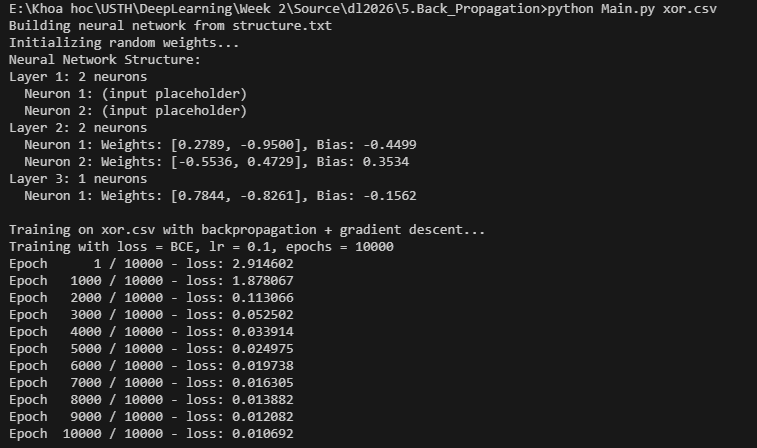
\includegraphics[width=0.9\textwidth]{Result_XOR_training.png}
    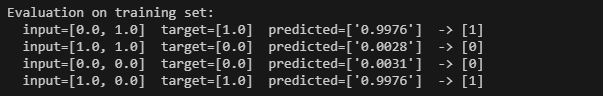
\includegraphics[width=0.9\textwidth]{Result_XOR_predictions.png}    
    \caption{Training log for XOR -- loss decrease over epochs and final predictions.}
    \label{fig:xor-train}
\end{figure}

\begin{figure}[H]
    \centering
    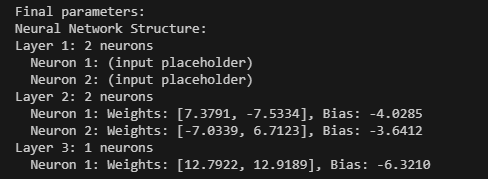
\includegraphics[width=0.9\textwidth]{Result_XOR_parameters.png}
    \caption{Final weights and bias for the XOR network after training.}
    \label{fig:xor-params}
\end{figure}

The trained weights are very different from the hand-crafted ones in lab 4, but the function it compute is still XOR. This show that the backpropagation can find a working solution by itself, without we set the parameters by hand.

\subsection{House price}

For a more realistic test, I also train the network on a small house price dataset. The CSV have a few input features (for example: area, number of rooms, $\dots$) and one output (the price). The price is normalized to $[0, 1]$ so the sigmoid output layer can fit it.

\begin{figure}[H]
    \centering
    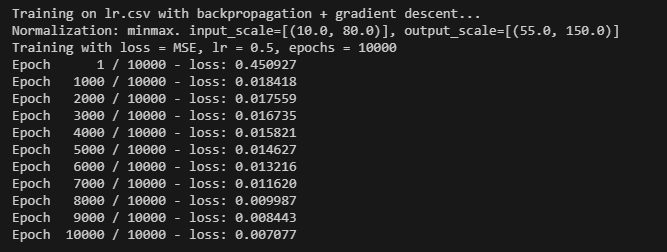
\includegraphics[width=0.9\textwidth]{Result_House_training.png}
    \caption{Training log for the house price dataset -- loss decrease over epochs.}
    \label{fig:house-train}
\end{figure}

\begin{figure}[H]
    \centering
    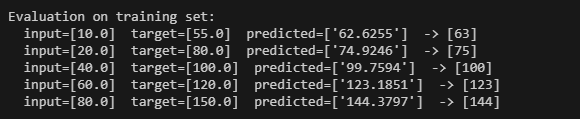
\includegraphics[width=0.9\textwidth]{Result_House_predictions.png}
    \caption{Predicted price vs target price on the training set.}
    \label{fig:house-pred}
\end{figure}

The loss go down steadily, which mean the same backpropagation code work for a regression-style task too, not only XOR.

\section{Conclusion}

The lab show that with only the standard Python library, we can implement backpropagation and gradient descent by ourself. The same small framework can learn XOR and also a small house price dataset, just by changing the CSV file and the \texttt{structure.txt}. The key part is the chain rule: each neuron know how to turn the upstream gradient into gradients for its own weights and bias, and how to pass the gradient further back.

\end{document}
